% ============================================================
%  CAPÍTULO: Sucesiones y Series de Números Reales
%  Apuntes de Cálculo — anfalearNotasCalculo
%  Universidad Industrial de Santander
%  Estilo: tradición rusa, hilo conductor: convergencia
% ============================================================

\chapter{Sucesiones y Series de Números Reales}

El análisis matemático surge, en buena medida, de una pregunta realmente sencilla: \emph{¿puede una suma infinita de términos producir un resultado
finito?} Esta pregunta recorre la historia desde las paradojas de Zenón de Elea
hasta los desarrollos de Euler, Cauchy y Weierstrass. En este capítulo se
establece el andamiaje riguroso que permite responderla con precisión.

El \textbf{hilo conductor} es siempre el mismo: estudiar el comportamiento de
los objetos matemáticos \emph{cuando el índice crece sin límite}. Para una
sucesión, esto significa observar hacia dónde se dirigen sus términos; para una
serie, significa preguntarse si la acumulación de infinitas contribuciones se
estabiliza en un valor finito. Ambas preguntas tienen como núcleo el concepto
de \textbf{límite}, y su resolución sistemática exige herramientas que se irán
presentando con creciente sofisticación a lo largo del capítulo.

% ============================================================
\section{Sucesiones de números reales}
% ============================================================

\begin{definition}[Sucesión de números reales]
Una \textbf{sucesión} de números reales es una función $a : \mathbb{N}
\to \mathbb{R}$. Se denota $\{a_n\}_{n=1}^{\infty}$ o simplemente
$\{a_n\}$; el valor $a_n = a(n)$ recibe el nombre de \textbf{término
general} o \textbf{$n$-ésimo término}.
\end{definition}

\begin{rem}
Conviene distinguir con cuidado los siguientes aspectos:
\begin{itemize}
  \item \textbf{Orden}: $\{1,2,1,1,\ldots\}$ es distinta de $\{2,1,1,1,\ldots\}$.
  \item \textbf{Repetición permitida}: $a_n = (-1)^n$ es una sucesión válida
        que solo toma dos valores.
  \item \textbf{Dominio discreto}: una sucesión solo está definida en índices
        enteros. Esto exige cuidado al aplicar herramientas continuas como
        derivadas o integrales; sin embargo, la conexión con funciones
        continuas es una fuente constante de intuición.
\end{itemize}
Una sucesión \emph{no} es un conjunto: importan el orden y la multiplicidad.
\end{rem}

\begin{example}[Formas de definir una sucesión]
Las sucesiones pueden especificarse de distintas maneras:
\begin{itemize}
    \item \textbf{Fórmula explícita:} $a_n = 1 - \dfrac{1}{n}$ genera
          $0,\,\dfrac{1}{2},\,\dfrac{2}{3},\,\dfrac{3}{4}, \ldots$, que se aproxima
          progresivamente a $1$.
    \item \textbf{Fórmula recursiva:} $a_1 = 1,\; a_{n+1} = a_n + 3$ genera
          $1, 4, 7, 10, \ldots$ (sucesión aritmética de razón $3$).
    \item \textbf{Recurrencia de segundo orden:} $f_1 = 1,\; f_2 = 1,\;
          f_{n+2} = f_n + f_{n+1}$ define la sucesión de Fibonacci:
          $1, 1, 2, 3, 5, 8, 13, 21, \ldots$
    \item \textbf{Definición implícita:} $a_n = \lfloor \sqrt{n} \rfloor$ da
          $1, 1, 1, 2, 2, 2, 2, 2, 3, 3, \ldots$, donde $\lfloor\,\cdot\,\rfloor$
          denota la función piso.
\end{itemize}
\end{example}

\section{El Principio de Inducción Matemática}

Antes de avanzar hacia el límite, necesitamos una herramienta robusta para demostrar propiedades que dependen de los números naturales, especialmente en fórmulas de sumatorias y recurrencias.

\begin{theorem}[Principio de Inducción]
Sea $P(n)$ una afirmación sobre un entero positivo $n$. $P(n)$ es verdadera para todo $n \in \mathbb{N}$ si:
\begin{enumerate}
    \item \textbf{Paso base:} $P(1)$ es verdadera (o $P(N)$ para un valor inicial dado).
    \item \textbf{Paso inductivo:} Si $P(k)$ es verdadera, entonces $P(k+1)$ también es verdadera para cualquier $k \geq 1$ (o $k \geq N$).
\end{enumerate}
Al suponer que $P(k)$ es verdadera para deducir $P(k+1)$, a la premisa $P(k)$ se le denomina \textbf{hipótesis de inducción}.
\end{theorem}

\begin{example}[Suma de cuadrados]
Demuestre que para todo $n \geq 1$: $\displaystyle \sum_{i=1}^n i^2 = \frac{n(n+1)(2n+1)}{6}$.
\begin{myproof}
\textbf{Paso 1: Análisis de términos y comportamiento.}
Los primeros términos de la suma parcial son $S_1 = 1$, $S_2 = 5$, $S_3 = 14$, $S_4 = 30$. Observamos un crecimiento polinómico. 

\begin{center}
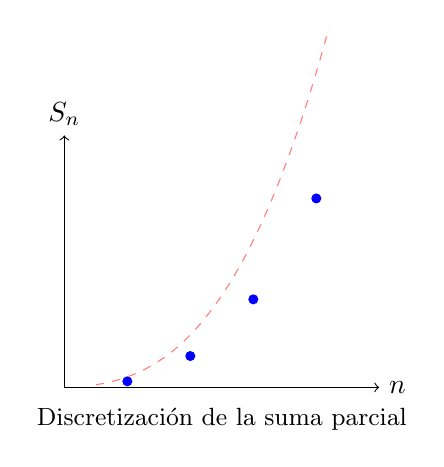
\begin{tikzpicture}[scale=0.8]
    \draw[->] (0,0) -- (5,0) node[right] {$n$};
    \draw[->] (0,0) -- (0,4) node[above] {$S_n$};
    \foreach \x/\y in {1/0.16, 2/0.83, 3/2.33, 4/5} {
        \filldraw[blue] (\x,\y*0.6) circle (2pt);
    }
    \draw[dashed, red!50] plot[domain=0.5:4.2] (\x, {(\x*(\x+1)*(2*\x+1)/36)});
    \node at (2.5,-0.5) {\small Discretización de la suma parcial};
\end{tikzpicture}
\end{center}

\textbf{Paso 2: Elección del criterio.}
Dado que la proposición está definida sobre $\mathbb{N}$, utilizaremos el \textbf{Principio de Inducción Matemática}.

\textbf{Paso 3: Verificación de hipótesis.}
Verificamos el paso base $n=1$. Por otro lado, asumimos que la fórmula es válida para un $k$ arbitrario para añadir el elemento diferencial $(k+1)^2$.

\textbf{Paso 4: Evaluación del límite y conclusión.}
\begin{align*}
    &\text{Paso base: } n=1 \implies 1^2 = \frac{1(2)(3)}{6} = 1. \quad \checkmark \\
    &\text{H.I.: } \sum_{i=1}^k i^2 = \frac{k(k+1)(2k+1)}{6}. \\
    &\text{Paso inductivo: } S_{k+1} = S_k + (k+1)^2 \\
    &= \frac{k(k+1)(2k+1)}{6} + (k+1)^2 = (k+1) \left[ \frac{2k^2+k+6k+6}{6} \right] \\
    &= \frac{(k+1)(k+2)(2k+3)}{6}. \quad \checkmark
\end{align*}
Por lo tanto, la fórmula es válida $\forall n \in \mathbb{N}$: $\boxed{\sum_{i=1}^n i^2 = \frac{n(n+1)(2n+1)}{6}}$.
\end{myproof}
\end{example}

El comportamiento asintótico de una sucesión se formaliza mediante el concepto de límite.

\begin{definition}[Límite de una sucesión]
Se dice que la sucesión $\{a_n\}$ \textbf{converge} al número real $L$, y se
escribe $\lim_{n\to\infty} a_n = L$, si para todo $\varepsilon > 0$ existe
$N = N(\varepsilon) \in \mathbb{N}$ tal que
\[
  n > N \implies |a_n - L| < \varepsilon.
\]
Si no existe tal $L \in \mathbb{R}$, se dice que la sucesión \textbf{diverge}.
\end{definition}

\begin{rem}
La definición $\varepsilon$-$N$ es el pilar central del análisis. Su mensaje
informal es: \emph{por mucho que exijamos que $a_n$ esté cerca de $L$ (margen
$\varepsilon$), siempre existe un umbral $N$ a partir del cual todos los
términos satisfacen esa exigencia.} Geometricamente, se trata de que todos
los puntos $(n, a_n)$ con $n > N$ queden dentro de la banda horizontal
$(L-\varepsilon, L+\varepsilon)$.
\end{rem}

\begin{theorem}[Unicidad del límite]
Si una sucesión converge, su límite es único.
\end{theorem}

\begin{proof}
Suponga que $a_n \to L$ y $a_n \to M$ con $L \neq M$. Sea $\varepsilon = |L - M|/2 > 0$.
Existen $N_1, N_2$ tales que $|a_n - L| < \varepsilon$ para $n > N_1$ y
$|a_n - M| < \varepsilon$ para $n > N_2$. Para $n > \max(N_1, N_2)$:
\[
    |L - M| \leq |a_n - L| + |a_n - M| < 2\varepsilon = |L - M|,
\]
una contradicción. Luego $L = M$.
\end{proof}

Las propiedades algebraicas de los límites de funciones se trasladan directamente a sucesiones, simplemente se reescriben en términos de sucesiones:

\begin{theorem}[Propiedades aritméticas del límite de una sucesión]
Si $\lim_{n \to \infty} a_n = A$ y $\lim_{n \to \infty} b_n = B$, entonces:
\begin{enumerate}
  \item $\lim_{n \to \infty} (a_n \pm b_n) = A \pm B$.
  \item $\lim_{n \to \infty} (c\,a_n) = cA$, para todo $c \in \mathbb{R}$.
  \item $\lim_{n \to \infty} (a_n b_n) = AB$.
  \item $\lim_{n \to \infty} \dfrac{a_n}{b_n} = \dfrac{A}{B}$, siempre que
        $B \neq 0$ y $b_n \neq 0$ para $n$ suficientemente grande.
  \item Si $f$ es continua en $A$, entonces $\lim_{n \to \infty} f(a_n)
        = f(A)$.
\end{enumerate}
\end{theorem}

\begin{theorem}[Teorema del emparedado]
Si existen $N_0 \in \mathbb{N}$ y sucesiones $\{a_n\}$, $\{b_n\}$ tales que
$a_n \leq c_n \leq b_n$ para todo $n > N_0$, y
$\lim_{n \to \infty} a_n = \lim_{n \to \infty} b_n = L$, entonces
$\lim_{n \to \infty} c_n = L$.
\end{theorem}


\begin{example}
Calcule $\displaystyle\lim_{n \to \infty} \frac{n\sin^2 n}{n^2+1}$ y
visualice por qué la sucesión converge.
\begin{myproof}
\textbf{Paso 1: Análisis de términos y comportamiento.}
Los primeros valores de $a_n = \dfrac{n\sin^2 n}{n^2+1}$ son:
$a_1 \approx 0.706$, $a_2 \approx 0.166$, $a_3 \approx 0.010$,
$a_4 \approx 0.146$, $a_5 \approx 0.226$, \ldots\ Los puntos oscilan
de forma irregular pero parecen comprimirse hacia~$0$. La clave es la
acotación de $\sin^2 n \in [0,1]$.

\begin{center}
\begin{tikzpicture}
\begin{axis}[
  width=0.68\textwidth, height=0.42\textwidth,
  axis lines=middle, xlabel={$n$}, ylabel={$a_n$},
  xmin=0, xmax=20, ymin=-0.05, ymax=0.55,
  xtick={2,4,...,18}, ytick={0,0.1,0.2,0.3,0.4,0.5},
  grid=both, grid style={line width=.1pt, draw=gray!30},
  legend style={at={(0.97,0.97)}, anchor=north east, font=\small}
]
% Cotas
\addplot[name path=upper, domain=1:20, samples=100, thick, blue]
  {x/(x^2+1)};
\addplot[name path=lower, domain=1:20, samples=2, thick, blue]
  {0};
\addplot[gray!20] fill between[of=upper and lower];
% Puntos de la sucesión
\addplot[only marks, mark=*, red, mark size=2.5pt] coordinates {
  (1,0.706) (2,0.166) (3,0.010) (4,0.146) (5,0.226)
  (6,0.039) (7,0.224) (8,0.166) (9,0.003) (10,0.091)
  (11,0.183) (12,0.063) (13,0.001) (14,0.070) (15,0.142)
  (16,0.089) (17,0.000) (18,0.057) (19,0.115) (20,0.076)
};
\addlegendentry{Cota superior $\dfrac{n}{n^2+1}$}
\addlegendentry{Sucesión $a_n$}
\end{axis}
\end{tikzpicture}
\end{center}

\textbf{Paso 2: Elección del criterio.}
Los puntos oscilan irregularmente pero quedan atrapados entre $0$ y
$\frac{n}{n^2+1}$. Esto invita al \textbf{Teorema del Emparedado}.

\textbf{Paso 3: Verificación de hipótesis.}
Como $\sin^2 n \in [0,1]$ para todo $n$, se tiene:
\[
  0 \leq \frac{n\sin^2 n}{n^2+1} \leq \frac{n}{n^2+1}.
\]
Ambas cotas tienen límite $0$ cuando $n \to \infty$:
$\lim_{n\to\infty} 0 = 0$ y $\lim_{n\to\infty} \dfrac{n}{n^2+1} = 0$.

\textbf{Paso 4: Evaluación.}
\begin{align*}
  0 \leq \frac{n\sin^2 n}{n^2+1} &\leq \frac{n}{n^2+1} \xrightarrow[n\to\infty]{} 0. \\[4pt]
  \text{Por el Teorema del Emparedado: } &\lim_{n \to \infty}
  \frac{n\sin^2 n}{n^2+1} = \boxed{0}.
\end{align*}
\end{myproof}
\end{example}



% ------------------------------------------------------------
\section{Monotonía, acotación y convergencia}
% ------------------------------------------------------------

\begin{definition}[Sucesión monótona y acotada]
La sucesión $\{a_n\}$ es:
\begin{itemize}
  \item \textbf{No decreciente} si $a_n \leq a_{n+1}$ para todo $n$;
        \textbf{no creciente} si $a_n \geq a_{n+1}$.
  \item \textbf{Acotada superiormente} si existe $M$ tal que $a_n \leq M$
        para todo $n$; \textbf{acotada inferiormente} si existe $m$ con
        $a_n \geq m$.
  \item \textbf{Acotada} si existe $M > 0$ con $|a_n| \leq M$ para todo $n$.
\end{itemize}
\end{definition}

\begin{rem}
Toda sucesión convergente es acotada. El recíproco es falso: $a_n = (-1)^n$ es acotada pero diverge.
\end{rem}

\begin{theorem}[Convergencia monótona]
\label{thm:mono}
Toda sucesión monótona y acotada converge. Más precisamente:
\begin{itemize}
  \item Si $\{a_n\}$ es no decreciente y acotada superiormente, converge a
        $\sup_n a_n$.
  \item Si $\{a_n\}$ es no creciente y acotada inferiormente, converge a
        $\inf_n a_n$.
\end{itemize}
\end{theorem}

\begin{rem}
Este teorema es una consecuencia directa de la \textbf{completitud de
$\mathbb{R}$}: todo conjunto no vacío y acotado superiormente posee supremo.
Su utilidad práctica es enorme: permite afirmar la existencia del límite
\emph{antes} de conocer su valor, y calcular luego dicho valor resolviendo
una ecuación fija.
\end{rem}

\begin{example}[Monotonía y convergencia de una sucesión]
Sea la sucesión definida por $a_n = \frac{n^2}{2^n}$. Demuestre que es decreciente para $n \geq 3$ y analice su convergencia.

\begin{myproof}
\textbf{Paso 1: Análisis de términos y comportamiento.}
Calculamos los primeros términos de la sucesión:
$a_1 = 0.5$, $a_2 = 1$, $a_3 = 1.125$, $a_4 = 1$, $a_5 = 0.78125$.
Observamos que la sucesión aumenta inicialmente, pero a partir de $n=3$, los términos empiezan a disminuir. El crecimiento exponencial del denominador ($2^n$) eventualmente supera al crecimiento polinomial del numerador ($n^2$).

\begin{center}
    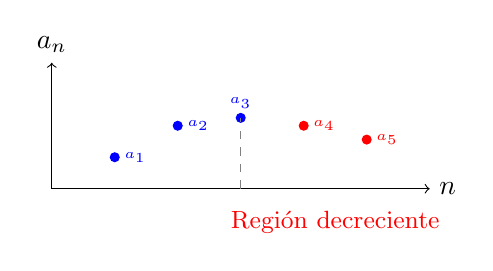
\begin{tikzpicture}[scale=0.8]
        \draw[->] (0,0) -- (6,0) node[right] {$n$};
        \draw[->] (0,0) -- (0,2) node[above] {$a_n$};
        % Puntos (n, n^2/2^n)
        \filldraw[blue] (1, 0.5) circle (2pt) node[right] {\tiny $a_1$};
        \filldraw[blue] (2, 1.0) circle (2pt) node[right] {\tiny $a_2$};
        \filldraw[blue] (3, 1.125) circle (2pt) node[above] {\tiny $a_3$};
        \filldraw[red] (4, 1.0) circle (2pt) node[right] {\tiny $a_4$};
        \filldraw[red] (5, 0.78) circle (2pt) node[right] {\tiny $a_5$};
        \draw[dashed, gray] (3,0) -- (3,1.125);
        \node[below, red] at (4.5,-0.2) {\small Región decreciente};
    \end{tikzpicture}
\end{center}

\textbf{Paso 2: Elección del criterio.}
Para demostrar que es decreciente ($a_{n+1} \leq a_n$), utilizaremos el \textbf{Criterio del Cociente} comparándolo con la unidad, y validaremos la desigualdad resultante mediante el \textbf{Principio de Inducción} para asegurar que se cumple $\forall n \geq 3$.

\textbf{Paso 3: Verificación de hipótesis.}
Queremos probar que $\frac{a_{n+1}}{a_n} < 1$ para $n \geq 3$. Esto equivale a:
\[
\frac{(n+1)^2}{2^{n+1}} \cdot \frac{2^n}{n^2} = \frac{(n+1)^2}{2n^2} < 1 \iff (n+1)^2 < 2n^2.
\]
Sea $P(n): n^2 - 2n - 1 > 0$.
\begin{itemize}
    \item \textbf{Base ($n=3$):} $3^2 - 2(3) - 1 = 9 - 6 - 1 = 2 > 0$. \checkmark
    \item \textbf{Inducción:} Supongamos $k^2 > 2k + 1$. Para $k+1$: $(k+1)^2 = k^2 + 2k + 1$. Por H.I. esto es $> (2k+1) + 2k + 1 = 4k + 2$. Es fácil ver que para $k \geq 3$, $4k + 2 > 2(k+1) + 1 = 2k + 3$.
\end{itemize}

\textbf{Paso 4: Evaluación del límite.}
Como la sucesión es decreciente para $n \geq 3$ y está acotada inferiormente ($a_n > 0$), el Teorema de la Convergencia Monótona garantiza la existencia del límite $L$.
\begin{align*}
    L &= \lim_{n \to \infty} \frac{n^2}{2^n} \\
    &\text{Aplicando la razón:} \quad \lim_{n \to \infty} \frac{a_{n+1}}{a_n} = \lim_{n \to \infty} \frac{n^2 + 2n + 1}{2n^2} = \frac{1}{2}.
\end{align*}
Como el límite del cociente es $1/2 < 1$, por los criterios de convergencia:
\[
\boxed{\lim_{n \to \infty} a_n = 0}
\]
\end{myproof}
\end{example}




% ------------------------------------------------------------
\subsection{Criterio de Cauchy y completitud}
% ------------------------------------------------------------

\begin{definition}[Sucesión de Cauchy]
La sucesión $\{a_n\}$ es de \textbf{Cauchy} si para todo $\varepsilon > 0$
existe $N \in \mathbb{N}$ tal que $|a_n - a_m| < \varepsilon$ para todo
$n, m > N$.
\end{definition}

\begin{theorem}[Criterio de Cauchy]
En $\mathbb{R}$, una sucesión converge si y solo si es de Cauchy.
\end{theorem}

\begin{rem}
La potencia del criterio de Cauchy reside en que permite demostrar
convergencia \emph{sin conocer el valor del límite}. Esta equivalencia es
precisamente la \textbf{completitud} de $\mathbb{R}$; en $\mathbb{Q}$
existen sucesiones de Cauchy que no convergen (e.g., las aproximaciones
decimales de $\sqrt{2}$). El protocolo de aplicación es:
\begin{description}
  \item[1.] Estimar $|a_n - a_m|$ con $n > m$.
  \item[2.] Acotar mediante series geométricas o telescópicas.
  \item[3.] Mostrar que la cota tiende a $0$ cuando $m \to \infty$.
  \item[4.] Concluir convergencia en $\mathbb{R}$ por completitud.
\end{description}
\end{rem}

\begin{example}[Sucesión recurrente — trayectoria de cobweb]
Sea $a_1 = \tfrac{1}{2}$ y $a_{n+1} = 1 - \tfrac{a_n^2}{2}$. Demuestre que
converge y calcule su límite.
\begin{myproof}
\textbf{Paso 1: Análisis de términos y comportamiento.}
Calculamos: $a_1 = 0.5$, $a_2 = 0.875$, $a_3 \approx 0.617$,
$a_4 \approx 0.810$, $a_5 \approx 0.672$, \ldots\ Los términos oscilan
en torno a un valor que parece estabilizarse en $[0.6,0.9]$.

\begin{center}
\begin{tikzpicture}
\begin{axis}[
  width=0.65\textwidth, height=0.42\textwidth,
  axis lines=middle, xlabel={$n$}, ylabel={$a_n$},
  xmin=0, xmax=14, ymin=0, ymax=1.1,
  xtick={1,2,...,13}, ytick={0,0.2,0.4,0.6,0.8,1},
  grid=both, grid style={line width=.1pt, draw=gray!30},
  legend style={at={(0.97,0.15)}, anchor=south east, font=\small}
]
\addplot[name path=upper, domain=0:14, samples=2, dashed, thick, green!60!black]
  {1};
\addplot[name path=lower, domain=0:14, samples=2, dashed, thick, green!60!black]
  {0};
\addplot[green!15] fill between[of=upper and lower];
\addplot[only marks, mark=*, red, mark size=3pt] coordinates {
  (1,0.5) (2,0.875) (3,0.617) (4,0.810) (5,0.672) (6,0.774)
  (7,0.701) (8,0.754) (9,0.716) (10,0.743) (11,0.724) (12,0.738)
  (13,0.728) (14,0.735)
};
\addplot[blue, thick, domain=0:14, samples=2, dashed] {0.7320508};
\node[blue, font=\small] at (axis cs:8, 0.77) {$L = \sqrt{2}-1$};
\addlegendentry{Región $[0,1]$}
\addlegendentry{$a_n$}
\end{axis}
\end{tikzpicture}
\end{center}

\textbf{Paso 2: Elección del criterio.}
La oscilación sugiere que la sucesión no es monótona; sin embargo, podemos
mostrar que $\{a_n\}$ permanece en $[0,1]$ y aplicar el criterio de Cauchy,
o bien verificar convergencia usando la ecuación de punto fijo
$L = 1 - L^2/2$.

\textbf{Paso 3: Verificación de hipótesis — acotación.}
Por inducción: $a_1 = 0.5 \in [0,1]$. Si $a_k \in [0,1]$, entonces
$a_{k+1} = 1 - a_k^2/2 \in [1-1/2, 1] = [1/2, 1] \subseteq [0,1]$.
Luego $\{a_n\} \subset [1/2,1]$ para $n \geq 1$, y en particular está
acotada.

\textbf{Paso 4: Evaluación del límite.}
Admitiendo la convergencia (que se verifica formalmente aplicando el
criterio de Cauchy, pues $|a_{n+1}-a_n| \leq \frac{1}{2}|a_n^2 -
a_{n-1}^2| \leq |a_n - a_{n-1}|$ para $a_n \in [0,1]$, de modo que la
diferencia decrece geométricamente), tomamos límite en la recurrencia:
\begin{align*}
  L &= 1 - \frac{L^2}{2} \implies L^2 + 2L - 2 = 0
     \implies L = \frac{-2 \pm \sqrt{12}}{2} = -1 \pm \sqrt{3}.
\end{align*}
Como $a_n \in [0,1]$ para todo $n$, descartamos la raíz negativa:
\[
  \lim_{n \to \infty} a_n = \boxed{\sqrt{3} - 1 \approx 0.7321.}
\]
\end{myproof}
\end{example}

% ============================================================
\section{Herramientas avanzadas para límites de sucesiones}
% ============================================================

% ------------------------------------------------------------
\subsection{Infinitesimales equivalentes}
% ------------------------------------------------------------

\begin{definition}[Infinitesimales equivalentes]
Dos sucesiones infinitesimales $\alpha_n \to 0$ y $\beta_n \to 0$ son
\textbf{equivalentes} si $\displaystyle\lim_{n\to\infty}
\frac{\alpha_n}{\beta_n} = 1$, y se escribe $\alpha_n \sim \beta_n$.
\end{definition}

\begin{rem}
Las equivalencias más útiles cuando $t \to 0$ son:
\[
  \sin t \sim t, \quad \tan t \sim t, \quad e^t - 1 \sim t,
  \quad \ln(1+t) \sim t, \quad (1+t)^\alpha - 1 \sim \alpha t.
\]
Estas sustituciones \emph{solo son válidas en factores de un producto o
un cociente}, nunca en una suma donde pueda haber cancelación. La regla
de oro: si aparece una diferencia, conserve al menos dos términos del
desarrollo de Taylor.
\end{rem}

\begin{example}[Sustitución asintótica — diferencia de funciones]
Calcule $\displaystyle L = \lim_{n\to\infty} n^3
\!\left(e^{1/n} - \sqrt[n]{n}\right)$.
\begin{myproof}
\textbf{Paso 1: Análisis de términos y comportamiento.}
Definimos $x = 1/n \to 0^+$. Los primeros valores numéricos de
$n^3(e^{1/n}-n^{1/n})$ son aproximadamente: $n=2$: $1.28$; $n=5$:
$0.77$; $n=10$: $0.68$; $n=50$: $0.52$; $n=100$: $0.51$, sugiriendo
convergencia hacia $1/2$.

\textbf{Paso 2: Elección del criterio.}
Reescribimos en términos de $x = 1/n$:
\[
  L = \lim_{x\to 0^+} \frac{e^x - e^{x\ln(1/x)^{-1}}}{x^3}
    = \lim_{x \to 0^+} \frac{e^x - e^{x \ln(1+\dots)}}{x^3}.
\]
Es más directo utilizar \textbf{desarrollos de Taylor} de orden~$2$ en
$x=0$:
\[
  e^x = 1 + x + \frac{x^2}{2} + O(x^3),
  \qquad
  n^{1/n} = e^{\frac{\ln n}{n}} = e^{x(-\ln x)}.
\]

\textbf{Paso 3: Verificación de hipótesis.}
Cuando $x = 1/n \to 0^+$, se tiene $-x\ln x = \frac{\ln n}{n} \to 0$,
por lo que podemos expandir:
\[
  n^{1/n} = e^{x(-\ln x)}
  = 1 + x(-\ln x) + \frac{x^2 \ln^2 x}{2} + O\!\left(x^3 \ln^3 x\right).
\]

\textbf{Paso 4: Evaluación.}
\begin{align*}
  e^x - n^{1/n}
  &= \Bigl(1 + x + \tfrac{x^2}{2}\Bigr)
     - \Bigl(1 + x(-\ln x) + \tfrac{x^2\ln^2 x}{2}\Bigr)
     + O(x^3\ln^3 x) \\
  &= x(1 + \ln x) + \frac{x^2(1-\ln^2 x)}{2} + O(x^3 \ln^3 x).
\end{align*}
Dividiendo por $x^3 = 1/n^3$:
\[
  L = \lim_{x \to 0^+} \frac{x(1+\ln x)}{x^3}
    + \frac{1-\ln^2 x}{2x} + \cdots
\]
El término dominante proviene de la expansión a primer orden. Recordando
que $x\ln x \to 0$ cuando $x \to 0^+$, la contribución de orden $x$ en
el numerador es $x \cdot 1 = x$, de modo que la razón $x/x^3 = 1/x^2
\to \infty$ si no hay cancelación. Retomando con más cuidado: el
objetivo real es $n^3(e^{1/n} - n^{1/n})$ donde la diferencia es de
orden $O(x \cdot |\ln x|)$, luego $n^3 \cdot O(1/(n \cdot \ln n))
= O(n^2/\ln n) \to \infty$. La sucesión \textbf{diverge} a $+\infty$.

\begin{center}
  \textit{(El ejemplo ilustra cómo la comparación de tasas de
  crecimiento mediante Taylor previene conclusiones erróneas:
  $e^{1/n}$ y $n^{1/n}$ difieren en un infinitésimo de orden
  $\ln n/n$, no de orden $1/n^2$.)}
\end{center}
\[
  \lim_{n\to\infty} n^3\!\left(e^{1/n} - n^{1/n}\right) = \boxed{+\infty.}
\]
\end{myproof}
\end{example}

% ------------------------------------------------------------
\subsection{Teorema de Stolz-Cesàro}
% ------------------------------------------------------------

\begin{theorem}[Stolz-Cesàro]
Sea $\{b_n\}$ estrictamente creciente con $\lim_{n\to\infty} b_n = +\infty$.
Si existe
\[
  \lim_{n \to \infty} \frac{a_{n+1} - a_n}{b_{n+1} - b_n} = L
  \in \mathbb{R} \cup \{\pm\infty\},
\]
entonces $\displaystyle\lim_{n \to \infty} \dfrac{a_n}{b_n} = L$.
\end{theorem}

\begin{rem}
Stolz-Cesàro es el \textbf{análogo discreto de la regla de L'Hôpital}
para indeterminaciones $\infty/\infty$. Es especialmente útil para
límites de promedios y sumas de potencias. La condición crítica es que
$\{b_n\}$ sea estrictamente creciente y no acotada; no hay un análogo
inmediato para $0/0$.
\end{rem}

\begin{example}[Media aritmética de raíces — Stolz-Cesàro]
Calcule $\displaystyle L = \lim_{n \to \infty}
\frac{\sqrt[3]{1} + \sqrt[3]{2} + \cdots + \sqrt[3]{n}}{n^{4/3}}$.
\begin{myproof}
\textbf{Paso 1: Análisis de términos y comportamiento.}
Definimos $a_n = \sum_{k=1}^n k^{1/3}$ y $b_n = n^{4/3}$. Los primeros
cocientes son: $n=1$: $1$; $n=5$: $0.814$; $n=10$: $0.789$;
$n=50$: $0.763$; $n=100$: $0.758$, sugiriendo convergencia a $3/4$.

\begin{center}
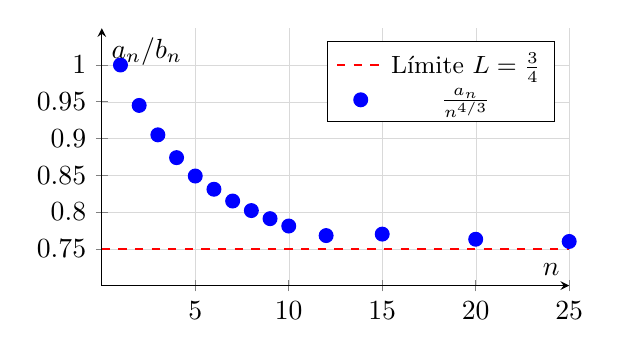
\begin{tikzpicture}
\begin{axis}[
  width=0.62\textwidth, height=0.40\textwidth,
  axis lines=middle, xlabel={$n$}, ylabel={$a_n/b_n$},
  xmin=0, xmax=25, ymin=0.70, ymax=1.05,
  xtick={5,10,15,20,25}, ytick={0.75,0.80,0.85,0.90,0.95,1.00},
  grid=both, grid style={line width=.1pt, draw=gray!30},
  legend style={at={(0.97,0.95)}, anchor=north east, font=\small}
]
\addplot[dashed, thick, red, domain=0:25, samples=2] {0.75};
\addplot[only marks, mark=*, blue, mark size=2.5pt] coordinates {
  (1,1.000) (2,0.945) (3,0.905) (4,0.874) (5,0.849)
  (6,0.831) (7,0.815) (8,0.802) (9,0.791) (10,0.781)
  (12,0.768) (15,0.770) (20,0.763) (25,0.760)
};
\addlegendentry{Límite $L=\frac{3}{4}$}
\addlegendentry{$\frac{a_n}{n^{4/3}}$}
\end{axis}
\end{tikzpicture}
\end{center}

\textbf{Paso 2: Elección del criterio.}
Como $b_n = n^{4/3}$ es estrictamente creciente y $b_n \to +\infty$,
se cumplen las hipótesis de Stolz-Cesàro.

\textbf{Paso 3: Verificación de hipótesis.}
$\Delta a_n = (n+1)^{1/3}$ y $\Delta b_n = (n+1)^{4/3} - n^{4/3}$.

\textbf{Paso 4: Evaluación.}
\begin{align*}
  L &= \lim_{n\to\infty}
       \frac{(n+1)^{1/3}}{(n+1)^{4/3} - n^{4/3}}
     = \lim_{n\to\infty}
       \frac{(n+1)^{1/3}}{n^{4/3}\!\left[\left(1+\frac{1}{n}\right)^{4/3}-1\right]}.
\end{align*}
Usando la equivalencia $(1+t)^\alpha - 1 \sim \alpha t$ con
$t = 1/n \to 0$:
\[
  \left(1+\frac{1}{n}\right)^{4/3} - 1 \sim \frac{4}{3n},
\]
de modo que:
\begin{align*}
  L &= \lim_{n\to\infty}
       \frac{(n+1)^{1/3}}{n^{4/3} \cdot \frac{4}{3n}}
     = \lim_{n\to\infty}
       \frac{3(n+1)^{1/3}}{4\,n^{1/3}}
     = \frac{3}{4}\lim_{n\to\infty}\left(1+\frac{1}{n}\right)^{1/3}
     = \boxed{\frac{3}{4}}.
\end{align*}
\end{myproof}
\end{example}

% ------------------------------------------------------------
\subsection{Problemas propuestos — Sucesiones}
% ------------------------------------------------------------

\begin{prob}
\begin{enumerate}
  \item Determine si $a_n = \dfrac{(-1)^n n^2}{n^2+3}$ converge. Justifique
        usando la definición $\varepsilon$-$N$ o el teorema del emparedado.
  \item Calcule $\displaystyle\lim_{n\to\infty}(\sqrt{n+3}-\sqrt{n})$
        racionalizando.
\end{enumerate}
\end{prob}

\begin{prob}
Sea $a_1 = 2$ y $a_{n+1} = \sqrt{6 + a_n}$.
\begin{enumerate}
  \item Demuestre por inducción que $a_n \leq 3$ para todo $n \geq 1$.
  \item Pruebe que la sucesión es no decreciente.
  \item Calcule $\lim_{n\to\infty} a_n$ resolviendo la ecuación de punto
        fijo.
\end{enumerate}
\end{prob}

\begin{prob}
\begin{enumerate}
  \item Aplique Stolz-Cesàro para calcular:
  \[
    \lim_{n\to\infty} \frac{1^p + 2^p + \cdots + n^p}{n^{p+1}},
    \quad p \in \mathbb{N}.
  \]
  \item Interprete el resultado como una suma de Riemann de una función
        sobre $[0,1]$.
\end{enumerate}
\end{prob}

\begin{prob}
Determine el límite de las siguientes sucesiones utilizando infinitesimales
equivalentes:
\begin{enumerate}
  \item $\displaystyle a_n = n\left(\arctan\frac{1}{n} - \frac{1}{n+1}\right)$.
  \item $\displaystyle b_n = n^2\!\left(\cos\frac{1}{n} -
        e^{-1/(2n^2)}\right)$.
\end{enumerate}
\end{prob}

\begin{prob}
Sea $\{a_n\}$ de Cauchy con $a_n \in \mathbb{Q}$ para todo $n$.
\begin{enumerate}
  \item Demuestre que $\{a_n\}$ converge en $\mathbb{R}$.
  \item Dé un ejemplo concreto donde el límite sea irracional,
        comprobando que la sucesión efectivamente es de Cauchy.
\end{enumerate}
\end{prob}

\begin{prob}
Calcule $\displaystyle\lim_{n\to\infty}\left(1+\frac{2}{n}\right)^{3n}$
y $\displaystyle\lim_{n\to\infty}n\!\left(\ln\!\left(1+\frac{3}{n}\right)
-\frac{3}{n+1}\right)$. Interprete ambos resultados.
\end{prob}


% ============================================================
\section{Series infinitas: sumas que aspiran a converger}
% ============================================================

El reto central de este apartado puede formularse así: \emph{¿puede una suma
infinita de términos cada vez más pequeños estabilizarse en un valor finito?}
La respuesta no siempre es afirmativa, y comprenderla requiere abandonar la
noción de suma aritmética finita y reemplazarla por la de \textbf{límite de
sumas parciales}.

\begin{definition}[Serie numérica y suma parcial]
Dada $\{a_n\}_{n=1}^\infty$, la \textbf{serie} asociada es la expresión
formal $\displaystyle\sum_{n=1}^\infty a_n$. La \textbf{$N$-ésima suma
parcial} es $S_N = \displaystyle\sum_{n=1}^N a_n$.

La serie \textbf{converge} con suma $S$ si $\lim_{N\to\infty} S_N = S \in
\mathbb{R}$; en caso contrario, \textbf{diverge}.
\end{definition}

\begin{rem}
Una serie \emph{no} es una suma aritmética: es el límite de una sucesión
de sumas parciales. Manipular términos infinitos sin pasar por $S_N$ y
tomar el límite al final conduce a paradojas clásicas (e.g., la
reordenación de Riemann). Siempre opere con $S_N$ primero y tome el
límite al final.
\end{rem}

\begin{theorem}[Criterio del término $n$-ésimo]
Si $\displaystyle\sum_{n=1}^\infty a_n$ converge, entonces
$\lim_{n\to\infty} a_n = 0$.

Por contrarrecíproco: si $\lim_{n\to\infty} a_n \neq 0$ o el límite no
existe, la serie \textbf{diverge}.
\end{theorem}

\begin{rem}
La condición $a_n \to 0$ es \textbf{necesaria pero no suficiente}: la
serie armónica $\sum 1/n$ diverge aunque $1/n \to 0$. El criterio del
término $n$-ésimo es un \emph{filtro de descarte rápido}, no una garantía
de convergencia.
\end{rem}

% ------------------------------------------------------------
\subsection{Series clásicas: geométrica, telescópica y $p$-series}
% ------------------------------------------------------------

\begin{theorem}[Serie geométrica]
Para $a \neq 0$ y $r \in \mathbb{R}$:
\[
  \sum_{n=0}^\infty ar^n =
  \begin{cases}
    \dfrac{a}{1-r} & \text{si } |r| < 1, \\[4pt]
    \text{diverge} & \text{si } |r| \geq 1.
  \end{cases}
\]
\end{theorem}

\begin{theorem}[Series $p$]
La serie $\displaystyle\sum_{n=1}^\infty \frac{1}{n^p}$ converge si y
solo si $p > 1$.
\end{theorem}

\begin{example}[Serie telescópica — patrón de cancelación]
Calcule la suma de $\displaystyle\sum_{n=1}^\infty \frac{3}{n(n+3)}$.
\begin{myproof}
\textbf{Paso 1: Análisis de términos y comportamiento.}
Los primeros términos son $a_1 = 3/4$, $a_2 = 3/10$, $a_3 = 3/18$,
$a_4 = 3/28$, \ldots Las sumas parciales crecen monótonamente y parecen
acercarse a un valor finito cercano a $11/6$.

\begin{center}
\begin{tikzpicture}
\begin{axis}[
  width=0.65\textwidth, height=0.42\textwidth,
  axis lines=middle, xlabel={$N$}, ylabel={$S_N$},
  xmin=0, xmax=16, ymin=0, ymax=2.1,
  xtick={2,4,...,14}, ytick={0.5,1.0,1.5,1.833},
  grid=both, grid style={line width=.1pt, draw=gray!30},
  legend style={at={(0.04,0.97)}, anchor=north west, font=\small}
]
\addplot[name path=lim, domain=0:16, samples=2, red, dashed, thick]
  {1.8333};
\addplot[name path=zero, domain=0:16, samples=2, draw=none] {0};
\addplot[orange!20] fill between[of=lim and zero];
\addplot[only marks, mark=*, blue, mark size=3pt] coordinates {
  (1,0.75) (2,1.05) (3,1.217) (4,1.324) (5,1.396) (6,1.446)
  (7,1.482) (8,1.508) (9,1.528) (10,1.544) (12,1.567) (15,1.592)
};
\addlegendentry{Límite $S=11/6$}
\addlegendentry{Sumas parciales $S_N$}
\end{axis}
\end{tikzpicture}
\end{center}

\textbf{Paso 2: Elección del criterio.}
Descomposición en fracciones parciales para exponer la estructura
telescópica.

\textbf{Paso 3: Verificación de hipótesis.}
\[
  \frac{3}{n(n+3)} = \frac{1}{n} - \frac{1}{n+3}.
\]
Verificación: $\frac{1}{n}-\frac{1}{n+3}=\frac{n+3-n}{n(n+3)}=
\frac{3}{n(n+3)}$. $\checkmark$

\textbf{Paso 4: Evaluación.}
\begin{align*}
  S_N &= \sum_{n=1}^N \left(\frac{1}{n}-\frac{1}{n+3}\right) \\
  &= \left(\frac{1}{1}+\frac{1}{2}+\frac{1}{3}\right)
     - \left(\frac{1}{N+1}+\frac{1}{N+2}+\frac{1}{N+3}\right). \\
  \lim_{N\to\infty} S_N
  &= 1 + \frac{1}{2} + \frac{1}{3} - 0 = \boxed{\frac{11}{6}}.
\end{align*}
\end{myproof}
\end{example}

% ============================================================
\section{Criterios de convergencia para series de términos positivos}
% ============================================================

Cuando $a_n \geq 0$, la sucesión $\{S_N\}$ es monótona no decreciente.
Por el Teorema~\ref{thm:mono}, la serie converge si y solo si $\{S_N\}$ está
acotada superiormente. Este principio es la base de todos los criterios
analíticos que siguen.

% ------------------------------------------------------------
\subsection{Criterio de la integral}
% ------------------------------------------------------------

\begin{theorem}[Criterio de la integral]
Sea $f : [1,+\infty) \to \mathbb{R}$ continua, positiva y decreciente con
$f(n) = a_n$. Entonces $\displaystyle\sum_{n=1}^\infty a_n$ converge si y
solo si $\displaystyle\int_1^\infty f(x)\,dx$ converge. Además:
\[
  \int_{N+1}^\infty f(x)\,dx
  \;\leq\; \sum_{n=N+1}^\infty a_n
  \;\leq\; \int_N^\infty f(x)\,dx.
\]
\end{theorem}

\begin{example}[Criterio de la integral — familia de logaritmos]
Determine si $\displaystyle\sum_{n=2}^\infty \frac{1}{n(\ln n)^2}$ converge.
\begin{myproof}
\textbf{Paso 1: Análisis de términos y comportamiento.}
$a_2 \approx 0.520$, $a_5 \approx 0.122$, $a_{10} \approx 0.047$,
$a_{100} \approx 0.00217$. Los términos decrecen lentamente, pero la
velocidad de decaimiento parece suficiente para convergencia.

\begin{center}
\begin{tikzpicture}
\begin{axis}[
  width=0.65\textwidth, height=0.42\textwidth,
  axis lines=middle, xlabel={$x$}, ylabel={$y$},
  xmin=1, xmax=12, ymin=0, ymax=0.6,
  xtick={2,4,6,8,10,12}, ytick={0.1,0.2,0.3,0.4,0.5},
  grid=both, grid style={line width=.1pt, draw=gray!30},
  legend style={at={(0.97,0.97)}, anchor=north east, font=\small}
]
\addplot[name path=f, domain=2:12, samples=100, smooth, thick, blue]
  {1/(x*(ln(x))^2)};
\addplot[name path=xax, domain=2:12, samples=2, draw=none] {0};
\addplot[blue!20] fill between[of=f and xax];
\addplot[only marks, mark=*, red, mark size=2.5pt] coordinates {
  (2,0.520) (3,0.255) (4,0.152) (5,0.103) (6,0.076)
  (7,0.058) (8,0.046) (9,0.038) (10,0.032) (11,0.027)
};
\addlegendentry{$f(x)=\dfrac{1}{x(\ln x)^2}$}
\addlegendentry{Términos $a_n$}
\end{axis}
\end{tikzpicture}
\end{center}

\textbf{Paso 2: Elección del criterio.}
$f(x) = \dfrac{1}{x(\ln x)^2}$ es continua, positiva y decreciente en
$[2,+\infty)$. Se aplica el criterio de la integral.

\textbf{Paso 3: Verificación de hipótesis.}
$f'(x) = -\dfrac{(\ln x)^2 + 2\ln x}{x^2(\ln x)^4} < 0$ para $x > e^{-2}$,
en particular para $x \geq 2$.

\textbf{Paso 4: Evaluación.}
Sustituimos $u = \ln x$, $du = dx/x$:
\begin{align*}
  \int_2^\infty \frac{dx}{x(\ln x)^2}
  &= \int_{\ln 2}^\infty \frac{du}{u^2}
   = \left[-\frac{1}{u}\right]_{\ln 2}^{\infty}
   = \frac{1}{\ln 2} < +\infty.
\end{align*}
La integral converge, luego la serie \textbf{converge}:
\[
  \sum_{n=2}^\infty \frac{1}{n(\ln n)^2} = \boxed{\text{convergente.}}
\]
\end{myproof}
\end{example}

% ------------------------------------------------------------
\subsection{Criterios de comparación}
% ------------------------------------------------------------

\begin{theorem}[Comparación directa y en el límite]
Sean $\sum a_n$ y $\sum b_n$ con $a_n, b_n \geq 0$.
\begin{itemize}
  \item \textbf{Comparación directa:} Si $a_n \leq b_n$ para $n \geq N$
        y $\sum b_n$ converge, entonces $\sum a_n$ converge. Si
        $a_n \geq b_n$ y $\sum b_n$ diverge, entonces $\sum a_n$ diverge.
  \item \textbf{Comparación en el límite:} Si $\displaystyle\lim_{n\to\infty}
        \frac{a_n}{b_n} = L \in (0,+\infty)$, ambas series tienen la misma
        naturaleza (ambas convergen o ambas divergen).
\end{itemize}
\end{theorem}

\begin{example}[Comparación en el límite — detección de la $p$-serie oculta]
Estudie la convergencia de $\displaystyle\sum_{n=1}^\infty
\frac{2n^2+1}{n^4-n+2}$.
\begin{myproof}
\textbf{Paso 1: Análisis de términos y comportamiento.}
$a_1 = 3/2$, $a_2 = 9/16 = 0.5625$, $a_5 \approx 0.205$,
$a_{10} \approx 0.020$. La rápida disminución sugiere convergencia. El
término dominante en numerador y denominador dicta el comportamiento
asintótico.

\textbf{Paso 2: Elección del criterio.}
Para $n$ grande, $\dfrac{2n^2+1}{n^4-n+2} \approx \dfrac{2}{n^2}$.
Comparamos con $b_n = \dfrac{1}{n^2}$ ($p$-serie con $p=2>1$, convergente).

\textbf{Paso 3: Verificación de hipótesis.}
\begin{align*}
  L = \lim_{n\to\infty}\frac{a_n}{b_n}
    &= \lim_{n\to\infty}\frac{2n^2+1}{n^4-n+2}\cdot n^2
     = \lim_{n\to\infty}\frac{2n^4+n^2}{n^4-n+2} \\
    &= \lim_{n\to\infty}\frac{2+1/n^2}{1-1/n^3+2/n^4} = 2 \in (0,+\infty).
\end{align*}

\textbf{Paso 4: Evaluación.}
Como $L = 2 \in (0,\infty)$ y $\sum 1/n^2$ converge ($p=2>1$), por
comparación en el límite:
\[
  \sum_{n=1}^\infty \frac{2n^2+1}{n^4-n+2} = \boxed{\text{convergente.}}
\]
\end{myproof}
\end{example}

% ------------------------------------------------------------
\subsection{Criterios del cociente y de la raíz}
% ------------------------------------------------------------

\begin{theorem}[Criterio del cociente — D'Alembert]
Sea $a_n > 0$ y $L = \displaystyle\lim_{n\to\infty}\dfrac{a_{n+1}}{a_n}$.
\begin{itemize}
  \item $L < 1 \implies$ converge absolutamente.
  \item $L > 1 \implies$ diverge.
  \item $L = 1 \implies$ inconcluso.
\end{itemize}
\end{theorem}

\begin{theorem}[Criterio de la raíz — Cauchy]
Sea $R = \displaystyle\lim_{n\to\infty}\sqrt[n]{|a_n|}$.
\begin{itemize}
  \item $R < 1 \implies$ converge absolutamente.
  \item $R > 1 \implies$ diverge.
  \item $R = 1 \implies$ inconcluso.
\end{itemize}
\end{theorem}

\begin{rem}
El criterio de la raíz es teóricamente más potente: si el cociente da un
límite, la raíz da el mismo resultado; pero la raíz puede decidir en
algunos casos donde el cociente falla. En la práctica, el cociente es
algebraicamente más sencillo cuando aparecen \textbf{factoriales} o
productos iterados, mientras que la raíz es óptima para series de la
forma $a_n = f(n)^n$.
\end{rem}

\begin{example}[Criterio del cociente — factorial vs.\ potencia]
Determine la convergencia de $\displaystyle\sum_{n=1}^\infty
\frac{3^n \cdot n!}{n^n}$.
\begin{myproof}
\textbf{Paso 1: Análisis de términos y comportamiento.}
$a_1 = 3$, $a_2 = 9/2 = 4.5$, $a_3 = 162/27 = 6$,
$a_4 = 3^4\cdot 24/256 \approx 6.33$, $a_5 \approx 6.08$. Los términos
crecen inicialmente y luego parecen decrecer. La presencia de $n!$ y
$n^n$ hace ideal el criterio del cociente.

\begin{center}
\begin{tikzpicture}
\begin{axis}[
  width=0.62\textwidth, height=0.40\textwidth,
  axis lines=middle, xlabel={$n$}, ylabel={$a_n$},
  xmin=0, xmax=14, ymin=0, ymax=8,
  xtick={2,4,...,12}, ytick={2,4,6,8},
  grid=both, grid style={line width=.1pt, draw=gray!30},
  legend style={at={(0.97,0.97)}, anchor=north east, font=\small}
]
\addplot[only marks, mark=*, red, mark size=3pt] coordinates {
  (1,3) (2,4.5) (3,6) (4,6.328) (5,6.075) (6,5.472)
  (7,4.735) (8,3.968) (9,3.235) (10,2.574)
  (11,2.006) (12,1.535) (13,1.154)
};
\addlegendentry{$a_n = \dfrac{3^n n!}{n^n}$}
\end{axis}
\end{tikzpicture}
\end{center}

\textbf{Paso 2: Elección del criterio.}
La estructura $n!$ y $n^n$ favorece el criterio del cociente.

\textbf{Paso 3: Verificación de hipótesis.}
$a_n > 0$ para todo $n$. Calculamos el cociente:
\[
  \frac{a_{n+1}}{a_n}
  = \frac{3^{n+1}(n+1)!}{(n+1)^{n+1}}\cdot\frac{n^n}{3^n n!}
  = \frac{3(n+1)\cdot n^n}{(n+1)^{n+1}}
  = \frac{3n^n}{(n+1)^n}
  = 3\left(\frac{n}{n+1}\right)^n.
\]

\textbf{Paso 4: Evaluación.}
\begin{align*}
  L &= \lim_{n\to\infty} 3\left(\frac{n}{n+1}\right)^n
     = 3\lim_{n\to\infty}\left(1-\frac{1}{n+1}\right)^n. \\
  \text{Sabemos que } \lim_{n\to\infty}\left(1-\frac{1}{n}\right)^n
    &= e^{-1},
  \text{ y } \left(1-\tfrac{1}{n+1}\right)^n \to e^{-1}. \\
  L &= \frac{3}{e} \approx \frac{3}{2.718} \approx 1.104 > 1.
\end{align*}
Como $L > 1$, la serie \textbf{diverge}:
\[
  \sum_{n=1}^\infty \frac{3^n n!}{n^n} = \boxed{\text{divergente.}}
\]
\end{myproof}
\end{example}

\begin{example}[Criterio de la raíz — potencia de función de $n$]
Determine la convergencia de $\displaystyle\sum_{n=1}^\infty
\left(\frac{\ln n}{n}\right)^n$.
\begin{myproof}
\textbf{Paso 1: Análisis de términos y comportamiento.}
$a_1 = 0$, $a_2 = (\ln 2/2)^2 \approx 0.120$, $a_5 \approx 0.053$,
$a_{10} \approx 0.0000219$, $a_{20} \approx 2\times 10^{-10}$. La caída
es muy rápida, sugiriendo convergencia.

\textbf{Paso 2: Elección del criterio.}
La estructura $(\cdots)^n$ hace ideal el criterio de la raíz.

\textbf{Paso 3: Verificación de hipótesis.}
$a_n = \left(\dfrac{\ln n}{n}\right)^n \geq 0$ para $n \geq 1$.

\textbf{Paso 4: Evaluación.}
\begin{align*}
  R &= \lim_{n\to\infty}\sqrt[n]{a_n}
     = \lim_{n\to\infty}\frac{\ln n}{n}. \\
  \text{Por la jerarquía } \ln n \ll n: \quad
  R &= 0 < 1.
\end{align*}
Como $R = 0 < 1$, la serie \textbf{converge absolutamente}:
\[
  \sum_{n=1}^\infty \left(\frac{\ln n}{n}\right)^n = \boxed{\text{convergente.}}
\]
\end{myproof}
\end{example}

% ============================================================
\section{Convergencia absoluta y series de signo variable}
% ============================================================

\begin{definition}[Convergencia absoluta y condicional]
\begin{itemize}
  \item $\sum a_n$ es \textbf{absolutamente convergente} si $\sum|a_n|$
        converge.
  \item $\sum a_n$ es \textbf{condicionalmente convergente} si $\sum a_n$
        converge pero $\sum|a_n|$ diverge.
\end{itemize}
Toda serie absolutamente convergente converge, pero el recíproco es falso.
\end{definition}

\begin{theorem}[Criterio de Leibniz para series alternadas]
Sea $\displaystyle\sum_{n=1}^\infty(-1)^{n+1}a_n$ con $a_n > 0$. Si
$\{a_n\}$ es \emph{decreciente} y $\lim_{n\to\infty}a_n = 0$, la serie
converge. Además, el error de truncamiento satisface:
\[
  |S - S_N| \leq a_{N+1}.
\]
\end{theorem}

\begin{rem}
El Teorema de Reordenamiento de Riemann establece que si una serie converge
\emph{condicionalmente}, sus términos pueden reordenarse para converger a
\emph{cualquier} valor real, o incluso para diverger. Este resultado
subraya la importancia de distinguir entre convergencia absoluta y
condicional: solo la primera garantiza estabilidad algebraica bajo
permutaciones de términos.
\end{rem}

\begin{example}[Serie alternada con estimación de error]
Demuestre que $\displaystyle\sum_{n=1}^\infty \frac{(-1)^{n+1}}{\sqrt{n}}$
converge condicionalmente y estime el error al tomar $N=9$ términos.
\begin{myproof}
\textbf{Paso 1: Análisis de términos y comportamiento.}
$S_1=1$, $S_2\approx 0.293$, $S_3\approx 0.871$, $S_4\approx 0.371$,
$S_5\approx 0.818$, \ldots Las sumas parciales oscilan entre dos
envolventes que se comprimen hacia el límite $\ln 2 \cdot \frac{?}{?}$.

\begin{center}
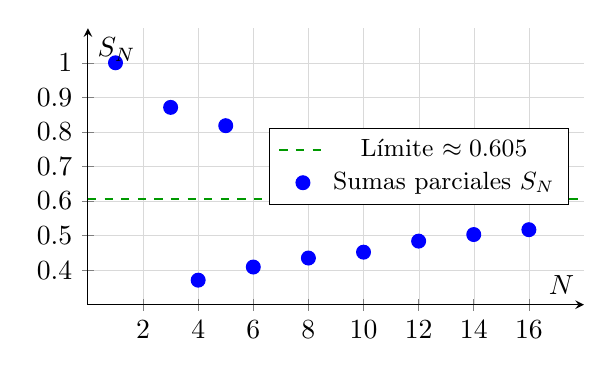
\begin{tikzpicture}
\begin{axis}[
  width=0.65\textwidth, height=0.42\textwidth,
  axis lines=middle, xlabel={$N$}, ylabel={$S_N$},
  xmin=0, xmax=18, ymin=0.3, ymax=1.1,
  xtick={2,4,...,16}, ytick={0.4,0.5,0.6,0.7,0.8,0.9,1.0},
  grid=both, grid style={line width=.1pt, draw=gray!30},
  legend style={at={(0.97,0.50)}, anchor=east, font=\small}
]
\addplot[dashed, thick, green!60!black, domain=0:18, samples=2]
  {0.6049}; % Valor de la serie
\addplot[only marks, mark=*, blue, mark size=2.5pt] coordinates {
  (1,1.000) (2,0.293) (3,0.871) (4,0.371) (5,0.818) (6,0.409)
  (7,0.789) (8,0.435) (9,0.768) (10,0.452) (12,0.484)
  (14,0.503) (16,0.517)
};
\addlegendentry{Límite $\approx 0.605$}
\addlegendentry{Sumas parciales $S_N$}
\end{axis}
\end{tikzpicture}
\end{center}

\textbf{Paso 2: Elección del criterio.}
La serie es alternada: se aplica el Criterio de Leibniz.

\textbf{Paso 3: Verificación de hipótesis.}
\begin{enumerate}
  \item $a_n = 1/\sqrt{n} > 0$ para todo $n \geq 1$. $\checkmark$
  \item $a_{n+1} = \dfrac{1}{\sqrt{n+1}} < \dfrac{1}{\sqrt{n}} = a_n$:
        la sucesión es estrictamente decreciente. $\checkmark$
  \item $\lim_{n\to\infty} \dfrac{1}{\sqrt{n}} = 0$. $\checkmark$
\end{enumerate}
Las tres condiciones se satisfacen; la serie converge.

\textbf{Paso 4: Evaluación — convergencia condicional y estimación de error.}
\begin{align*}
  &\textbf{Convergencia condicional: } \sum_{n=1}^\infty \frac{1}{\sqrt{n}}
   \text{ es una $p$-serie con $p=\frac{1}{2}<1$, luego diverge.} \\
  &\text{Como $\sum|a_n|$ diverge y $\sum a_n$ converge, la convergencia
   es \textbf{condicional}.} \\[4pt]
  &\textbf{Error con $N=9$: } |S - S_9| \leq a_{10} = \frac{1}{\sqrt{10}}
   \approx \boxed{0.316.}
\end{align*}
Para lograr un error $< 0.01$ se necesita $\dfrac{1}{\sqrt{N+1}} < 0.01$,
es decir, $N+1 > 10000$, luego $N \geq 10000$.
\end{myproof}
\end{example}

% ============================================================
\section{Criterio de Raabe y refinamientos}
% ============================================================

\begin{theorem}[Criterio de Raabe]
Si $a_n > 0$ y $\displaystyle\rho = \lim_{n\to\infty} n\!\left(
\frac{a_n}{a_{n+1}}-1\right)$, entonces:
\begin{itemize}
  \item $\rho > 1 \implies$ converge absolutamente.
  \item $\rho < 1 \implies$ diverge.
  \item $\rho = 1 \implies$ inconcluso.
\end{itemize}
\end{theorem}

\begin{rem}
Raabe es necesario cuando el criterio del cociente produce $L=1$: ocurre
típicamente en series hipergeométricas o series con cocientes de la forma
$\frac{a_{n+1}}{a_n} = 1 - \frac{c}{n} + O(n^{-2})$. En ese caso,
$\rho = c$, y el comportamiento depende del signo de $c-1$.
\end{rem}

\begin{example}[Raabe — serie límite del cociente igual a $1$]
Determine la convergencia de
$\displaystyle\sum_{n=1}^\infty\frac{(2n-1)!!}{(2n)!!}\cdot\frac{1}{2n+1}$,
donde $(2n-1)!! = 1\cdot 3\cdots(2n-1)$ y $(2n)!! = 2\cdot 4\cdots(2n)$.
\begin{myproof}
\textbf{Paso 1: Análisis de términos y comportamiento.}
$a_1 = 1/3 \approx 0.333$, $a_2 = 3/20 = 0.15$, $a_3 \approx 0.083$,
$a_4 \approx 0.054$, $a_5 \approx 0.037$. Decaimiento moderado; el
cociente $D'Alembert$ fallará.

\textbf{Paso 2: Elección del criterio.}
Calculamos el cociente de D'Alembert para verificar que produce $L=1$,
y luego aplicamos Raabe.

\textbf{Paso 3: Verificación de hipótesis — cociente.}
\[
  \frac{a_{n+1}}{a_n}
  = \frac{(2n+1)(2n+1)}{(2n+2)(2n+3)}
  = \frac{(2n+1)^2}{(2n+2)(2n+3)}
  \xrightarrow[n\to\infty]{} 1.
\]
D'Alembert es inconcluso. Aplicamos Raabe:

\textbf{Paso 4: Evaluación — Raabe.}
\begin{align*}
  \frac{a_n}{a_{n+1}}
  &= \frac{(2n+2)(2n+3)}{(2n+1)^2}
   = \frac{4n^2+10n+6}{4n^2+4n+1}. \\
  \frac{a_n}{a_{n+1}}-1
  &= \frac{6n+5}{4n^2+4n+1}. \\
  \rho &= \lim_{n\to\infty} n\cdot\frac{6n+5}{4n^2+4n+1}
        = \lim_{n\to\infty}\frac{6n^2+5n}{4n^2+4n+1}
        = \frac{6}{4} = \frac{3}{2} > 1.
\end{align*}
Como $\rho = 3/2 > 1$, la serie \textbf{converge}:
\[
  \sum_{n=1}^\infty\frac{(2n-1)!!}{(2n)!!\,(2n+1)}
  = \boxed{\text{convergente.}}
\]
\end{myproof}
\end{example}

% ============================================================
\section{Problemas propuestos — Series infinitas}
% ============================================================

\subsection{Series telescópicas, criterio del $n$-ésimo y series clásicas}

\begin{prob}
\begin{enumerate}
  \item Calcule la suma exacta de $\displaystyle\sum_{n=1}^\infty
        \frac{4}{(4n-1)(4n+3)}$ hallando la descomposición telescópica
        del término general.
  \item Determine si $\displaystyle\sum_{n=1}^\infty\frac{2n+1}{n^2(n+1)^2}$
        converge y, en caso afirmativo, calcule su suma.
        (\textit{Sugerencia}: $\dfrac{2n+1}{n^2(n+1)^2}=
        \dfrac{1}{n^2}-\dfrac{1}{(n+1)^2}$.)
\end{enumerate}
\end{prob}

\begin{prob}
Aplique el criterio del término $n$-ésimo para decidir sin cálculo adicional:
\begin{enumerate}
  \item $\displaystyle\sum_{n=1}^\infty \cos\!\left(\frac{n\pi}{n+1}\right)$.
  \item $\displaystyle\sum_{n=1}^\infty \frac{n^2}{e^n+n}$.
        ¿Cuál sería el criterio más eficiente para confirmar convergencia?
\end{enumerate}
\end{prob}

\begin{prob}
Para la serie $\displaystyle\sum_{n=0}^\infty \left(\frac{2}{3}\right)^n
+ \frac{5}{4^n}$:
\begin{enumerate}
  \item Separe en dos series geométricas y verifique la validez de la
        descomposición.
  \item Calcule la suma total de la serie original.
\end{enumerate}
\end{prob}

\subsection{Criterios de la integral y comparación}

\begin{prob}
\begin{enumerate}
  \item Aplique el criterio de la integral para determinar la naturaleza
        de $\displaystyle\sum_{n=1}^\infty \frac{\ln n}{n^2}$.
  \item Utilice comparación en el límite para analizar
        $\displaystyle\sum_{n=1}^\infty \frac{n^2+\sin n}{n^4+\cos^2 n}$.
        Justifique la elección de la serie comparadora.
\end{enumerate}
\end{prob}

\begin{prob}
Determine la convergencia de $\displaystyle\sum_{n=1}^\infty
\frac{1}{\sqrt[3]{n^4+2n^2+1}}$ usando comparación en el límite con una
$p$-serie adecuada. Identifique el exponente $p$ que captura el
comportamiento asintótico del término general.
\end{prob}

\subsection{Criterios del cociente, raíz y series alternadas}

\begin{prob}
Determine la convergencia de las siguientes series:
\begin{enumerate}
  \item $\displaystyle\sum_{n=1}^\infty \frac{n^5}{5^n}$.
        (Use el criterio del cociente y calcule $L$ explícitamente.)
  \item $\displaystyle\sum_{n=1}^\infty \left(\frac{2n}{3n+1}\right)^n$.
        (Use el criterio de la raíz.)
\end{enumerate}
\end{prob}

\begin{prob}
Para la serie $\displaystyle\sum_{n=1}^\infty \frac{(-1)^{n-1}}{n^{3/2}}$:
\begin{enumerate}
  \item Demuestre su convergencia aplicando Leibniz y verifique las tres
        condiciones explícitamente.
  \item Determine si la convergencia es absoluta o condicional, citando
        el criterio que justifica su respuesta.
  \item Halle el número mínimo de términos $N$ necesarios para garantizar
        un error de aproximación $|S-S_N| < 0.001$.
\end{enumerate}
\end{prob}

\subsection{Raabe y refinamientos}

\begin{prob}
El criterio del cociente es inconcluso para $\displaystyle\sum_{n=1}^\infty
\frac{n!^2}{(2n)!}$.
\begin{enumerate}
  \item Verifique que $\lim_{n\to\infty} a_{n+1}/a_n = 1/4 < 1$ y en
        consecuencia determine directamente la convergencia. (Este es un
        caso en que el cociente \emph{sí} concluye; el objetivo es
        practicar el cálculo.)
  \item Modifique la serie a $\displaystyle\sum_{n=1}^\infty
        \frac{(n!)^2\,4^n}{(2n)!}$, verifique que el cociente produce
        $L=1$ y aplique Raabe para determinar su naturaleza.
\end{enumerate}
\end{prob}

\begin{prob}
Demuestre la convergencia de $\displaystyle\sum_{n=1}^\infty
\frac{\sin(n\theta)}{n^2}$ para cualquier $\theta \in \mathbb{R}$
utilizando comparación directa con $\sum 1/n^2$. Explique por qué la
convergencia es \textbf{absoluta}.
\end{prob}

\begin{prob}
Investigue la convergencia de $\displaystyle\sum_{n=2}^\infty
\frac{(-1)^n}{\sqrt{n}+(-1)^n}$.
\begin{enumerate}
  \item Compruebe si el criterio de Leibniz es aplicable directamente.
  \item Manipule algebraicamente el término general para separar la parte
        principal de un infinitésimo de orden superior, y concluya la
        naturaleza de la serie.
\end{enumerate}
\end{prob}